%%%%%%%%%%%%%%%%%%%%%%%%%%%%%%%%%%%%%%%%%%%%%%%%%%%%%%%%%%%%%%%%%%%%%%%%%%%%%%%%
\section{Summary}

%%%%%%%%%%%%%%%%%%%%%%%%%%%%%%%%%%%%%%%%%%%%%%%%%%%%%%%%%%%%%%%%%%%%%%%%%%%%%%%%
\begin{frame}[fragile]
  \frametitle{Implementing \texttt{glob\_wildcards}}
  Remember?
  \begin{lstlisting}[language=Python,style=Python,basicstyle=\tiny]
glob_wildcards('books/{book}.txt')
  \end{lstlisting}
  \pause
  We can use this to get hold of the \texttt{\{book\}}-wildcard and assign this list to a variable in our workflow:
  \begin{lstlisting}[language=Python,style=Python,basicstyle=\tiny]
DATS = glob_wildcards('books/{book}.txt').book
  \end{lstlisting}
  \task{Create a rule \texttt{make\_archive}}
  \footnotesize
  Hints:
      \begin{itemize}
       \item to create an archive we can use: \texttt{tar -czvf zipf\_analysis.tar.gz <file1> <file2> <file3> ...}
       \item we may use the list \texttt{DATS} as input:
          \begin{lstlisting}[language=Python,style=Python,basicstyle=\tiny]
rule make_archive:
    input:
        expand('plots/{book}.dat', book=DATS)
          \end{lstlisting}
      \end{itemize}
\end{frame}

%%%%%%%%%%%%%%%%%%%%%%%%%%%%%%%%%%%%%%%%%%%%%%%%%%%%%%%%%%%%%%%%%%%%%%%%%%%%%%%%
\begin{frame}[fragile]
  \frametitle{The \texttt{all}}
  The UNIX-make system per default has an \texttt{all} rule - snakemake derives this philosohy to create a default target.
  \task{Create an \texttt{all} as the first rule to expect \texttt{zipf\_analysis.tar.gz} (our final output) as input.}
\end{frame}



%%%%%%%%%%%%%%%%%%%%%%%%%%%%%%%%%%%%%%%%%%%%%%%%%%%%%%%%%%%%%%%%%%%%%%%%%%%%%%%%
\begin{frame}[fragile]
  \frametitle{\HandsOn{Bring Everything Together!}} 
  \begin{enumerate}
   \item Finally, many Snakefiles define a default target called all as first target, that will build what the Snakefile has been written to build (e.g. in our case, the \texttt{.png} files and the \texttt{results.txt} file). Add an ``\texttt{all}'' target to your Snakefile (Hint: this rule \texttt{tar.gz} as dependency). With that in place, instead of running \texttt{snakemake <target>}, you should now run \texttt{snakemake}.
   \item Update your workflow to:
     \begin{itemize}
      \item Adjust the \texttt{plot\_count} rule to contain wildcards (look at the \texttt{make\_archive}) for to use \texttt{DATS}).
      \item Remove \texttt{zipf\_analysis.tar.gz} when \texttt{snakemake clean} is called.
      \item Add the plots to our tarball.
     \end{itemize}
  \end{enumerate}
\end{frame}


%%%%%%%%%%%%%%%%%%%%%%%%%%%%%%%%%%%%%%%%%%%%%%%%%%%%%%%%%%%%%%%%%%%%%%%%%%%%%%%%
\begin{frame}[fragile]
  \frametitle{The Solution}
  \begin{columns}
    \begin{column}{0.5\textwidth}
     \begin{lstlisting}[language=Python,style=Python,basicstyle=\tiny]
# our zipf analysis workflow
DATS = glob_wildcards('books/{book}.txt').book

rule all:
    input:
        'zipf_analysis.tar.gz'

# delete everything so we can re-run things
rule clean:
    shell:snakemake --rulegraph | dot -Tpng > mini_dag.png
        '''
        rm -rf results dats plots
        rm -f results.txt zipf_analysis.tar.gz
        '''

# count words in one of our "books"
rule count_words:
    input:
        book='books/{file}.txt'
    output: 'dats/{file}.dat'
    shell:  'python scripts/wordcount.py'
            ' -i {input.book} -o {output}'
    \end{lstlisting}
    \end{column}
    \begin{column}{0.5\textwidth}
      \begin{lstlisting}[language=Python,style=Python,basicstyle=\tiny]
# create a plot for each book
rule make_plot:
    input:
        book='dats/{file}.dat'
    output: 'plots/{file}.png'
    envmodules:
       'vis/matplotlib'
    shell:  'python scripts/plotcount.py'
            ' -i {input.book} -o {output}'

# generate summary table
rule zipf_test:
    input:
        books=expand('dats/{book}.dat', 
                     book=DATS)
    output: 'results.txt'
    shell:  'python scripts/zipf_test.py'
            ' {input.books} > {output}'

# create an archive with all of our results
rule make_archive:
    input:
        expand('plots/{book}.png', book=DATS),
        expand('dats/{book}.dat', book=DATS),
        'results.txt'
    output: 'zipf_analysis.tar.gz'
    shell: 'tar -czvf {output} {input}'
      \end{lstlisting}
    \end{column}
  \end{columns}
\end{frame}

%%%%%%%%%%%%%%%%%%%%%%%%%%%%%%%%%%%%%%%%%%%%%%%%%%%%%%%%%%%%%%%%%%%%%%%%%%%%%%%%
\begin{frame}[fragile]
  \frametitle{Using temporary and protected Files}
  In fact, \emph{all} our files are temporary (quickly produced and wrapped in a tarball). Hence, the could be delted after completion of the workflow. All intermediate files should be labelled temporary, e.\,g.:
  \begin{lstlisting}[language=Python,style=Python,basicstyle=\tiny]
rule count_words:
    input:
        book='books/{file}.txt'
    output: temp('dats/{file}.dat')
    shell:  'python scripts/wordcount.py'
            ' -i {input.book} -o {output}'
  \end{lstlisting}
  \pause
  Likewise, files can be protected from accidental deletion with the \texttt{protected} flag, e.\,g.:
  \begin{lstlisting}[language=Python,style=Python,basicstyle=\tiny]
rule make_plot:
    input:
        book='dats/{file}.dat'
    output: protected('plots/{file}.png')
    envmodules:
       'vis/matplotlib'
    shell:  'python scripts/plotcount.py'
            ' -i {input.book} -o {output}'
  \end{lstlisting}
\end{frame}

%%%%%%%%%%%%%%%%%%%%%%%%%%%%%%%%%%%%%%%%%%%%%%%%%%%%%%%%%%%%%%%%%%%%%%%%%%%%%%%%
\begin{frame}[fragile]
  \frametitle{\HandsOn{Plotting the Workflow}}
  \texttt{Snakemake} has a build-in plotting feature. Run 
  \begin{lstlisting}[language=Bash, style=Shell]
$ snakemake --rulegraph | dot -Tpng > <your_workflow.png>
  \end{lstlisting}
  to plot your workflow graph. And
  \begin{lstlisting}[language=Bash, style=Shell]
$ display <your_workflow.png>
  \end{lstlisting}
  to display the workflow.
\end{frame}

%%%%%%%%%%%%%%%%%%%%%%%%%%%%%%%%%%%%%%%%%%%%%%%%%%%%%%%%%%%%%%%%%%%%%%%%%%%%%%%%
\begin{frame}
  \frametitle{Your DAG:}
  \centering
  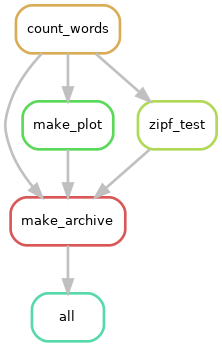
\includegraphics[width=0.4\textwidth]{workflows/complete_workflow.png}
\end{frame}


